\documentclass[a4paper, 12pt, oneside]{book}
\usepackage[T1]{fontenc}
\usepackage[utf8]{inputenc}
\usepackage[portuguese]{babel}
\usepackage{graphicx}
\usepackage{float}
\graphicspath{ {./imagens/} }
\usepackage[document]{ragged2e}
\usepackage{hyphenat}
\usepackage{lipsum}

\usepackage{xcolor}
\definecolor{cinza}{rgb}{0.5,0.5,0.5}

\usepackage[a4paper]{geometry}
\geometry{left=2.5cm}
\geometry{right=2.5cm}
\geometry{footskip=2.5cm}
\setlength{\parindent}{2em}
\setlength{\parskip}{1em}
\renewcommand{\baselinestretch}{1.5}

\usepackage[sfdefault]{roboto}

\usepackage[pagestyles]{titlesec}
\newpagestyle{meuestilo}{\setfoot[\thepage][][]{\fontfamily{Montserrat-TOsF}\selectfont\color{cinza} Projectus Invictus}{}{\fontfamily{Montserrat-TOsF}\selectfont\color{cinza}\thepage}}
\pagestyle{meuestilo}



\usepackage{sectsty}
\allsectionsfont{\fontfamily{Montserrat-TOsF}\selectfont\mdseries}
\chapterfont{\raggedleft\fontfamily{Montserrat-TOsF}\selectfont\mdseries}


\usepackage{etoolbox}
\AtBeginEnvironment{quote}{\large\itshape}

\title{Projectus Invictus}
\author{Lucas Costa}

\begin{document}
\maketitle

\chapter*{\underline{Introdução}}

A intenção deste e-book é de ajudar você, desenvolvedor, freelancer, engenheiro de software e programador, seja sozinho ou em equipe, a melhorar ou implementar um processo mais eficiente e rápido para produzir o seu software, desde as primeiras conversas com os interessados até a entrega final e após.

A Technologiká, hoje representada pelo seu fundador Lucas Costa (quem vos escreve), veio de um mundo acadêmico que caiu de paraquedas na indústria de desenvolvimento. Durante essa trajetória nos últimos anos, eu passei por várias dificuldades na hora de entender o que os clientes e superiores queriam que fosse desenvolvido, bem como exibir o andamento e realizar a entrega dos sistemas de uma maneira adequada, que também não consumisse mais tempo do que propriamente desenvolvendo.

Mas foi por meio destas experiências e dores que encontrei diversas ferramentas e metodologias que me ajudaram a fazer um trabalho de mais qualidade, que envolve o cliente do início ao fim e o deixa mais satisfeito, com um sistema que é mais a cara dele e tem de fato o que ele precisa pra solucionar o seu problema. São muitos mecanismos e métodos que, se aplicados da maneira correta e na sequência correta, produzem resultados poderosos, como: redução do tempo de desenvolvimento, aumento da qualidade, melhor comunicação com o cliente e aumento de sua satisfação. Fato é que é capaz de duplicar ou mais a velocidade de desenvolvimento e ainda reduzir pela metade o estresse do trabalho.

Na continuidade dessa jornada, percebi que muitos profissionais da nossa área passam pelas mesmas dificuldades que eu passei. Tanto colegas de estudo e até mesmo novos profissionais integrando minha equipe. Entendi que não é um conhecimento fácil de se obter, já que requereu muita experiência, erros e acertos, clientes perdidos e tempo perdido. A faculdade não me preparou pelo que estava por vir.

Por isso, entendi que tinha nas mãos uma missão: ajudar mais desenvolvedores a não passar por tantas dores desnecessárias. Portanto, a minha missão não é de ensinar a você técnicas de programação, códigos e linguagens, mas sim o que acontece além-código-fonte.

Há um ambiente externo à programação que muitos desconhecem e ignoram. Fato é que, se realmente conhecessem, seriam os mais felizes do mundo. E eu quero te levar um passo mais perto disso, ajudando você a se tornar:

\textbf{Um projetista Invictus.}

\noindent\makebox[\linewidth]{\rule{.5\paperwidth}{0.4pt}}

Quando falamos sobre o processo de produção de um software, uma das melhores formas de o dividir é em quatro partes:
\begin{itemize}
	\item Concepção: é aqui que começam as conversações com o seu cliente (entenda-se "cliente" como chefe, contratador, líder, ou seja, pra quem você vai fazer o sistema) para entender qual a ideia geral que o sistema vai atender, qual problema ele vai resolver;
	\item Elaboração: tendo uma noção clara do objetivo, esta fase é dedicada a documentar pontos chave do sistema. Não entenda "documentar" como o processo maçante de escrever textos que ninguém lê, os famosos "documentos de gaveta". A arte de documentar está em na capacidade de estabelecer maneiras visuais de representar a solução, tanto com protótipos, como por gráficos, ou até mesmo por textos;
	\item Construção: agora, mãos à massa! Com tudo bem arquitetado, o que falta é produzir o sistema de uma vez por todas. E nessa fase do processo, vários cuidados e técnicas devem ser aplicados;
	\item Implantação: quando se chega ao final da construção e desenvolvimento, é hora de implantar e disponibilizar a solução para o cliente. É o momento mais esperado por nós, portanto deve ser levado com atenção para que dê tudo certo.
\end{itemize}

Neste livro, trato cada uma dessas fases com detalhe, para que você não tenha dúvidas e sinta-se seguro em todas as fases de desenvolvimento do seu sistema. Tanto para um sistema que você está começando agora como para um que já está sendo desenvolvido, você pode inserir estas técnicas a partir de hoje no seu fluxo.

\chapter*{\underline{Concepção}}

O processo de concepção de um software pode ser bastante curto, pois é aqui onde você tem as primeiras conversas com seu cliente. Em casos esporádicos, pode levar mais tempo, quando por exemplo, ainda não se sabe bem o que vai construir, ou quando a comunicação com o cliente é lenta, dificultada.

Podemos dividir esse processo em duas fases, dependentes de contato com o cliente: o Contato Inicial e a Visualização do Sistema.

\section*{Contato Inicial}

Seja no ambiente empresarial, seja no contato direto, o começo de produção de um software sempre inicia com uma conversa, normalmente por parte do interessado. Ele vem com uma ideia, uma dúvida, às vezes com um sonho, com a crença inabalável que você é quem pode realizá-lo. Portanto, neste primeiro contato, seja polido e ouvinte. Não tire conclusões precipitadas.

Uma boa filosofia de vida e negócio que se aplica nesta fase do processo é acreditar nesta frase: "tudo é possível". Até mesmo as ideias mais mirabolantes podem se tornar em um sistema incrível como nenhum outro. Então aguarde com atenção e pense em soluções, não em dificuldades.

\begin{quote}
	\begin{flushright}
		Seja polido e ouvinte, não tire conclusões precipitadas. Lembre-se, "tudo é possível".
	\end{flushright}
\end{quote}

Entretanto, é imprescindível que você faça essas perguntas, para ajudar na delimitação do projeto:
\begin{itemize}
	\item Qual o objetivo do sistema/aplicativo/software?
	\item Qual problema ele resolve?
	\item Quem vai usar?
\end{itemize}

Essas questões serão feitas no futuro novamente para reafirmar o propósito do projeto, mas para uma primeira conversa já é o suficiente para se entender a ideia geral.

Depois deste primeiro contato, marque a próxima reunião o quanto antes com o seu cliente, para fazer a Visualização do Sistema. É importante que esse segundo encontro aconteça o quanto antes, para que as ideias e o interesse não se esfriem. Mas também, a depender de quão madura está a intenção, não é recomendado fazer isso imediatamente. Marque um horário, uma reunião, para se dedicar na próxima atividade, pois estará fundando os alicerces do projeto.


\section*{Visualização do Sistema}

Nesta fase do processo de Concepção, o seu objetivo é entender completamente qual a intenção ou objetivo do cliente: para quê ele quer um sistema? Como ele deve funcionar? Quem vai usar? Qual problema ele resolve? Tudo isso deve ser levantado nesse segundo momento, geralmente uma reunião presencial ou virtual. É um evento que marca que, realmente, o projeto vai ser desenvolvido! Porém, como ainda se trata de um processo inicial, não dá pra dizer que o que for dito aqui será uma verdade absoluta até o final do projeto. Na verdade, isso será definido na próxima fase, que é o processo de Elaboração.

A abordagem mais recomendada nesse tipo de conversa, para visualizar o sistema, é utilizar um esquema de mapa mental. Isso porque ele é simples, de fácil entendimento entre as duas partes: desenvolvedor e interessado. Ele funciona como uma união, uma ponte de comunicação entre o que o cliente quer e o que você vai precisar desenvolver.

Tente construir um modelo como este:

\begin{figure}[H]
	\caption{texto}
	\centering
	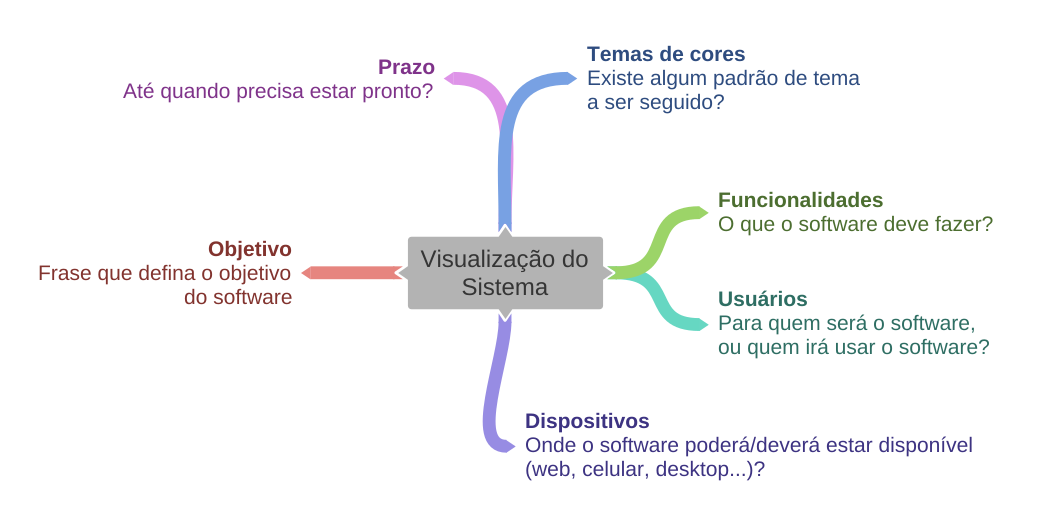
\includegraphics[width=0.8\textwidth]{Visualizao_do_Sistema.png}
\end{figure}

Explicando, desenhe um mapa cujo centro pode ser o nome do sistema, se já existir, ou um nome que o caracterize. Deste centro, devem sair seis ramificações seguindo a seguinte ordem:

\begin{itemize}
    \item \textbf{Objetivo:} constituído por uma frase curta, sucinta e objetiva que consiga descrever para quê vai servir esse sistema. Não precisa pensar ou elaborar muito, algo com as suas palavras ou as do cliente. Essa definição ajuda a responder as próximas questões;
    \item \textbf{Usuários:} quais são as pessoas, os atores, que vão usar esse sistema? Dessa ramificação devem sair os nomes de quem vai ter acesso ou quem vai efetivamente usar a aplicação;
    \item \textbf{Funcionalidades:} o que os usuários vão fazer? Quais ações eles terão disponíveis? As funcionalidades estão bastante ligadas aos usuários. Sua definição nesse momento também pode ser bastante rápida e enxuta, apenas para entender a serventia do sistema, alinhada ao objetivo já definido;
    \item \textbf{Dispositivos:} por onde os usuários vão acessar o sistema? Essa questão é importante para entender qual será a arquitetura do sistema, ou seja, qual tipo de tecnologia você vai precisar empregar no desenvolvimento da solução;
    \item \textbf{Prazo:} não precisa ser uma data bem definida, aqui é interessante ter noção do que o seu cliente espera, qual a expectativa dele. Esse também é um ponto importante de negociação, para se discutir desde o começo, evitando problemas futuros;
    \item \textbf{Temas de cores:} verifique se já existe alguma regra estilística que você deverá respeitar, se essa responsabilidade será de outra pessoa ou se fica de livre escolha sua.
\end{itemize}


Esse modelo de mapa pode e deve ser usado durante a conversa mesmo! Para desenhá-lo, a depender das circunstâncias, você pode usar caneta e papel, ou se possível, ferramentas de desenho digitais.

**Dica de ferramenta**
Para desenhar mapas mentais, eu gosto e utilizo o [Coggle](https://coggle.it/). É uma ferramenta gratuita e de fácil utilização para construção de mapas rápidos e bonitos.

**Exemplo de utilização**
[Neste vídeo](https://youtu.be/brfNJdwhlDA), eu explico como realizar esta etapa de Visualização do Sistema de maneira prática, simulando o levantamento de um aplicativo para alunos universitários.

Se durante a conversa você achar necessário, algo que pode ajudar é fazer um fluxo de operação, quando aplicável. O Fluxo de Operação é um desenho de telas, que mostra o caminhamento dentro do sistema e já ilustra e inclui algumas das funcionalidades. Por exemplo, algo mais ou menos assim:

\begin{figure}[H]
	\caption{texto}
	\centering
	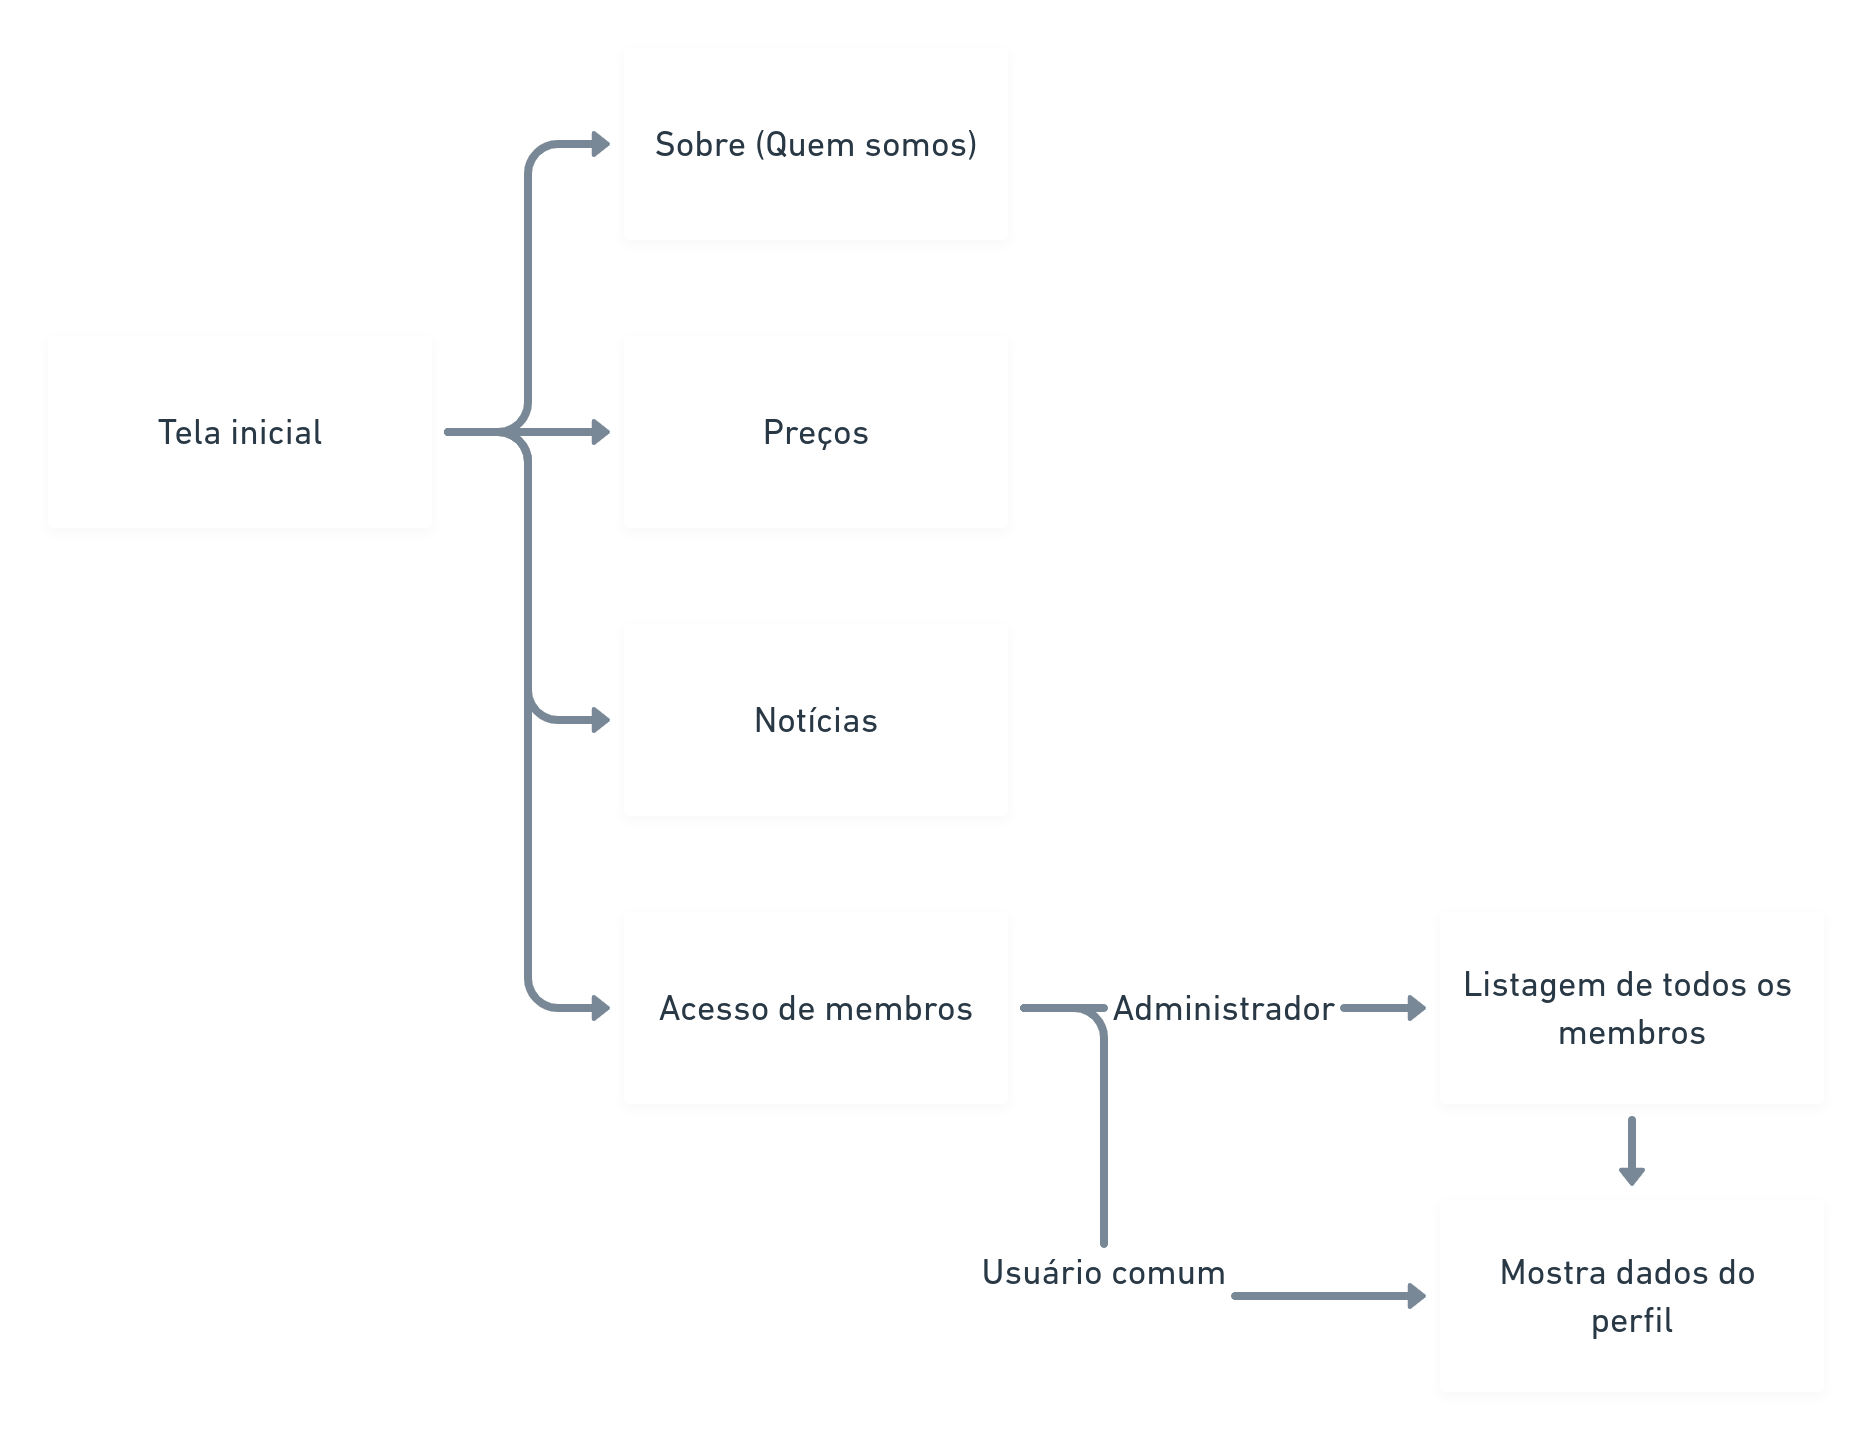
\includegraphics[width=0.8\textwidth]{Postagens2x.png}
\end{figure}

Esse fluxo pode representar a estrutura de um site simples, como um exemplo didático do que o Fluxo de Operação quer dizer.

**Dica de ferramenta**
Esse tipo de desenho fica legal quando se usa o [Whimsical](https://whimsical.com/). Similar em facilidade ao Coggle, mais voltado para esse tipo de desenho de fluxogramas e semelhantes.

Geralmente, com a conversa e com o mapa mental feito, você já tem material suficiente para seguir para a próxima fase. Interessante que a construção desse mapa também ajuda a levantar várias questões e dúvidas, e já responde muitas também. A carga de informação e esclarecimento é bastante alta.

Na próxima fase, começa a Elaboração do sistema. É um processo mais formal, que parte de você para o cliente, onde você vai mostrar e detalhar como o sistema vai funcionar, o que vai ser preciso pra isso, quanto tempo vai levar e quanto vai custar.

**Quanto tempo leva?**
A fase de concepção geralmente é bastante rápida. Pode acontecer tudo no mesmo dia. É recomendado que essa fase dure no mínimo dois dias, e no máximo duas semanas.

\end{document}
